%%%%%%%%%%%%%%%%%%%%%%% file moduleX_template.tex %%%%%%%%%%%%%%%%%
%
%
% This is a template for creating your papers for the course KRW
% It is based on the standard Latex template for Springer publications
% but contains a suggestion for the structure and some content of the
% paper.
%
% Please adapt this document wherever needed.
%
% For more information about the required Latex Style check the document
% typeinst.pdf in the StyleFiles directory.
%
%%%%%%%%%%%%%%%%%%%%%%%%%%%%%%%%%%%%%%%%%%%%%%%%%%%%%%%%%%%%%%%%%%%%%%%%%


\documentclass[runningheads,a4paper]{../../StyleFiles/llncs}

\usepackage{url}
\usepackage{graphicx}
\usepackage{amssymb}
\usepackage{listings}
\lstset{language=SQL,morekeywords={and, some, exactly}}


\newcommand{\keywords}[1]{\par\addvspace\baselineskip
\noindent\keywordname\enspace\ignorespaces#1}

\begin{document}

\mainmatter  % start of an individual contribution

% first the title is needed
\title{Data- and Ontology Paper: Quality Ontology for Handicap Parking Spots around Venues in Amsterdam}

% a short form should be given in case it is too long for the running head
\titlerunning{Data- and Ontology Paper}

% the name(s) of the author(s) follow(s) next
%
% NB: Chinese authors should write their first names(s) in front of
% their surnames. This ensures that the names appear correctly in
% the running heads and the author index.
%
\author{Alivanistos, Dimitris. \\ Baez, Selene. \\ Jemmett, Andrea. }
%
\authorrunning{Alivanistos, Dimitris. \\ Baez, Selene. \\ Jemmett, Andrea.}
% (feature abused for this document to repeat the title also on left hand pages)

% the affiliations are given next; don't give your e-mail address
% unless you accept that it will be published
\institute{\url{d.alivanistos@student.vu.nl} \and \url{s.baezsantamaria@student.vu.nl} \and \url{a.jemmett@student.vu.nl}}

\maketitle


\begin{abstract}
The abstract should summarize the contents of the paper and should
contain at least 70 and at most 150 words. It should be written using the
\emph{abstract} environment.
\end{abstract}


\section{Introduction}
Amsterdam, a busy and tourist city as it is, offers a variety of events throughout the year. As such, a relevant topic related to the previous is the accessibility the city provides for handicap people to attend such events. In particular, this project focuses on providing these users with a way to find Parking Slots when attending events in different venues in Amsterdam.

Though information about handicap parking slots in Amsterdam is public through the Municipality, the datasets are not structured in a human readable manner. Moreover, the link to venues and events is not well organized and has not been addressed in a user-friendly manner. To the extent of our knowledge, the application that gets closest to this description is the official website for Accessibility in Amsterdam, which still fails to provide with an easily searchable tool for finding handicap parking slots given an Event and/or Venue.
%TODO link to download datasets and to website.

This paper is an extension of the previous paper on Milestone 1, where we set up the project to solve the aforementioned problem, linking datasets from events at Theatres, and Museums and Galleries, to the Handicap Parking Slots dataset. In this paper the overall goal is to improve on the knowledge graph created for the application by creating an ontology that is formal yet intuitive for its potential users.

In the following section we further motivate the paper by providing concrete use cases that lead to a list of higher level requirements to be fulfilled by our project. Later, we describe an inspiration paper that guided us through the design of our ontology. We continue to describe our ontology, highlighting the major improvements from the knowledge graph in Milestone 1, followed up by evaluating the proposed ontology. Finally, some discussion provides with insights regarding the main contributions and future improvements on this project.

\section{Section 2 - Use Case and Requirements}
%\textit{Describe the use-case you have in mind that motivates the need for the ontology. This could be the original use case from milestone 1, but then you should explain why the schema you defined previously falls short. What requirements should the ontology meet? What is its intended scope.}
In order to better illustrate the motivation for this project we look back to the use cases from Milestone 1 to evaluate how well the current knowledge graph meets their needs. Next, we ambitiously create a couple more use cases to extend the potential uses of the application. We finalize by providing with a list of three specific requirements an ontology must meet to satisfy the users needs.

\subsection{Previous use cases}
\begin{enumerate}
	% Planning in advance
	\item John is in a wheelchair and wants to go to an exhibition in Van Gogh Museum Friday night. John likes to plan things in advance and would like to know where the parking slots closest to the theater are. \\
	The day before the show, John uses our application to find such parking slots and heads to the show confidently. 
	% Quick search once in the theater (on the fly)
	\item Peter broke his leg last month and his friends, as an attempt to cheer him up, invited him to come to a comedy show at the Comedy Cafe. He is quite late and he is rushing to find the closest parking slots. He quickly browses our application and finds an area with several parking slots. He drives in that direction hoping to find an available slot. 
	% Event manager
	\item Mary is an event organizer who wants to host an exhibition in a museum next month. She is looking for an accessible venue so she would like to see the distribution of parking slots around the main galleries in Amsterdam. She has a list of five places in mind and uses our application to explore and choose the best venue.
\end{enumerate}

\textbf{Why the previous schema falls short?}
John and Peter have to go through a long list of events till they find the exhibition or show they are attending. A new ontology that subdivides events into types helps him navigate the data more easily. 

\subsection{New use cases}

\begin{enumerate}
	% Search by interest
	\item Toribio is only interested in theatre plays. He is in a wheelchair and needs accessible parking spots to go to Theatres when he selects a play to watch. 
	% Search by area
	\item Chachita has appointments once every week at the Femme Amsterdam Hospital. She would like to look for events nearby to attend after her sessions. 
\end{enumerate}

\subsection{Requirements}

\begin{enumerate}
	\item Search by interest
	\item Detailed location information
	\item Detailed information about Parking Slots (size)
\end{enumerate}


\section{Section 3 - Related Work}
\textit{What other ontologies did you find that cover a similar domain. To what extent can they be reused. Have others (e.g. other students) developed similar datasets/ontologies that feed/meet your requirements, where do they fall short? Papers to look for are published at eg. ISWC, ESWC, EKAW and FOIS, or the Journal of Web Semantics, and the Semantic Web Journal.}

- Ontology for smart cities: \cite{komninos2015smart}. Heavily inspired by this paper for ontology design. 

- Our ontology fits in the broader schema of theirs. Specific for Handicap Parking Slots, Venues and Events. 


\section{Section 4 - Methodology}
\textit{Describe the methodology you followed for constructing the ontology. How did you guarantee that the ontology meets the needs and requirements of the use case? Have you used any existing design patterns, partial ontologies, competency questions etc.}

- Use of Protégé

- Iterative process.

- Subclasses, cardinality, object Properties

- Extensive use of powerful ontologies like dbo. Use of equivalence between dbo:Place and dbo:Location

\section{Section 5 - The Ontology}
\textit{Systematically describe the ontology and highlight the (interesting) design choices you had to make. Were there things you wanted to represent but couldn't given the limitations on the KR language?\footnote{If you do not encounter any limitations, you should be more ambitious about the model!} How did you work around these limitations? (integrity constraints, additional rules?) Describe how the ontology meets the 5 star model for Linked Vocabulary Use.}

%TODO insert image
\begin{figure}[h]
	\centering
	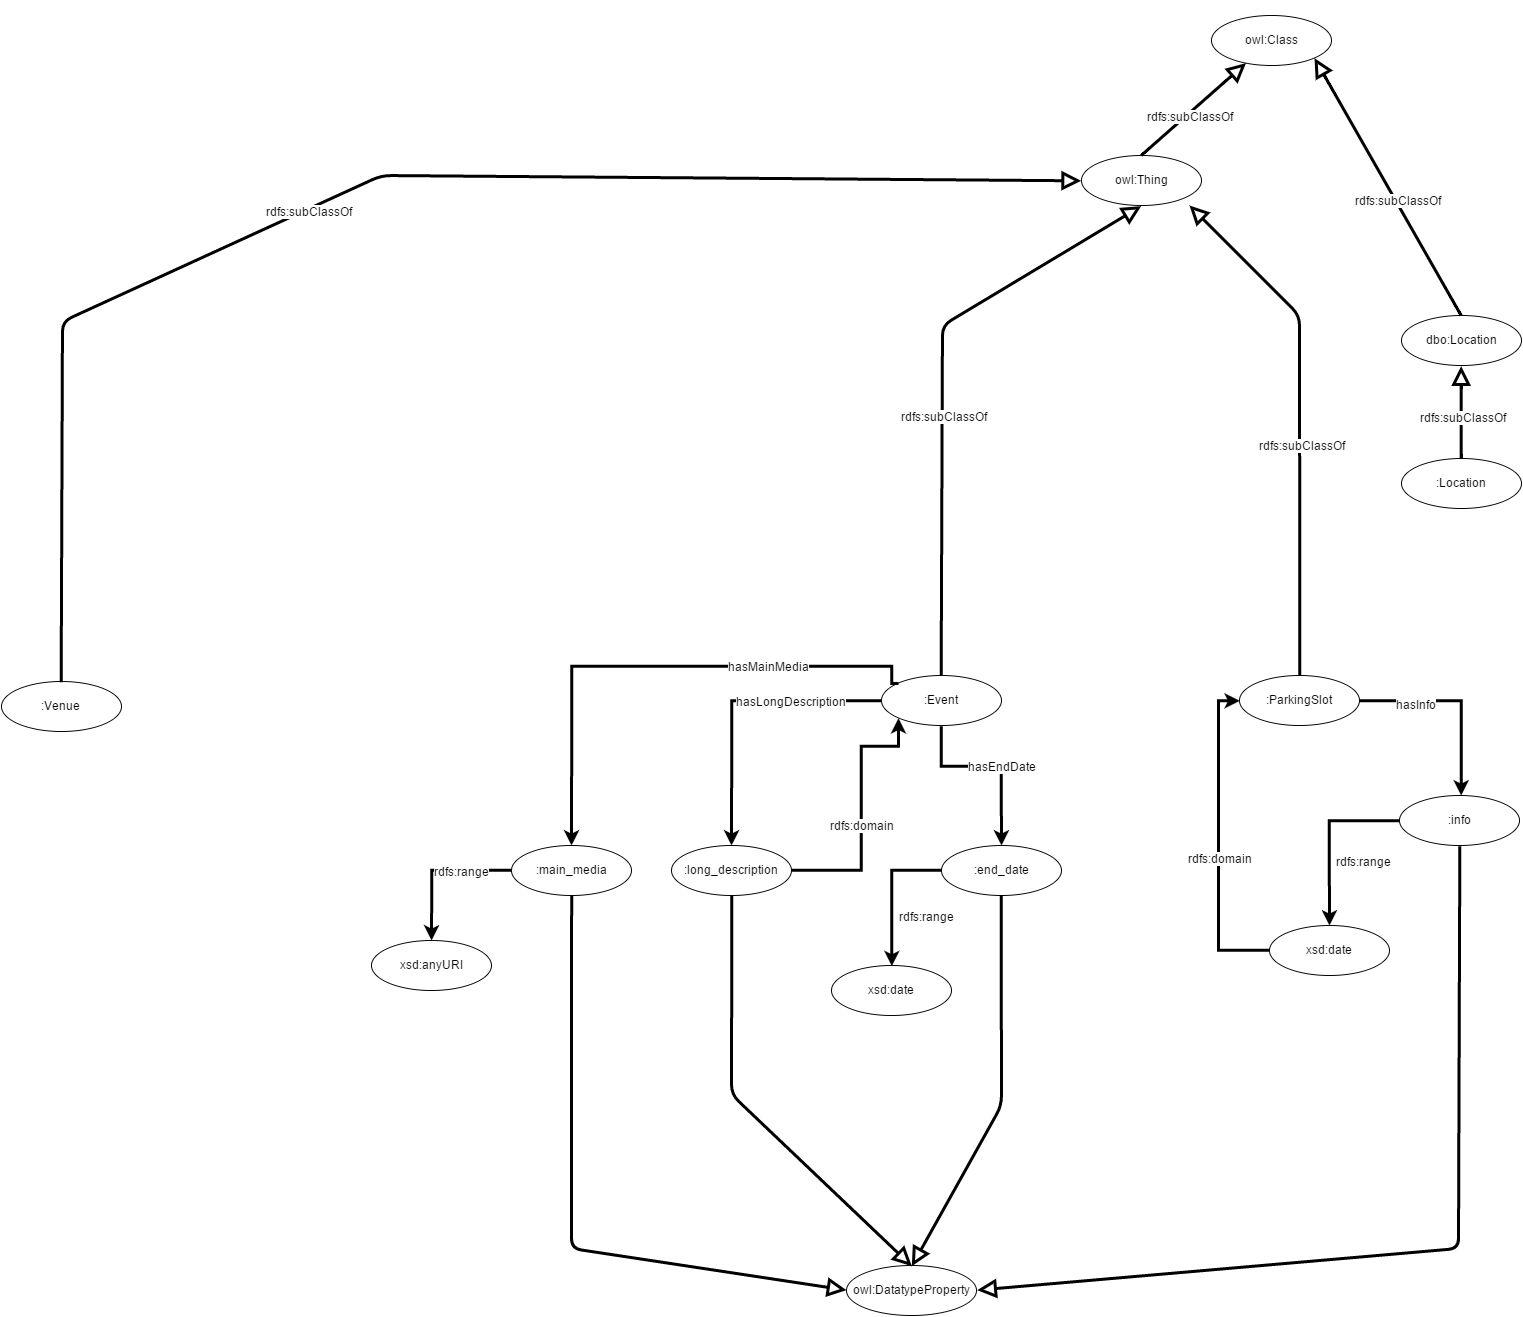
\includegraphics[width=.7\textwidth]{img/ontology.png}
	\caption{Visualization of the Ontology graph}
	\label{fig:ontology}
\end{figure}

\subsection{Entities}
- Now we have subclasses for each of the main type of classes we had before

- Events: into Plays and Exhibitions
- Venues into Theatres and Museums
- Parking Slot into Small Medium and Large

- First two distinctions come from the datasets themselves. The third one we created based on size. Parking Slot has datatype property quantity, which serves a a classifier

\begin{lstlisting}[captionpos=b, caption=Definition of Large Slot a subclass of Parking Slot, label=lst:owl, basicstyle=\ttfamily\small,frame=bt]
(dbo:location exactly 1 Location)
and (info exactly 1 xsd:string)
and (quantity exactly 1 xsd:unsignedInt)
\end{lstlisting}

- Our Location class extends dbo:Location class in the use of Borough

\subsection{Properties}

- Restrictions on datatype properties. Cardinalities are explicit, so that they reflect that an Event has only one Venue, for example

- Introduce 'Event venue' which has subproperties 'Exhibition Venue' and 'Play Venue' depending on their range. Also introduce its inverse 'Venue Events'

- We create a subproperty of dbo:location to be 'venue location'. We restrict dbo:location to have domain Parking Slots while 'venue location' has domain Venues. Both have Location as range.

- Properties for Borough, City and Country


\section{Section 6 - The Dataset}
\textit{Describe how you recasted the dataset(s) of the previous assignment to the new ontology (perhaps you found other datasets that you want to add). What did it take to do this? What metadata have you published alongside the dataset, and how did you generate it? (Provenance, VOID, etc.) Describe how your data meeds the 5 star model for Linked Data.}


\section{Section 7 - Evaluation}
\textit{Evaluate the ontology and dataset with respect to each other (does the ontology really sanction only the intended inference) and with respect to the requirements and use case (extend your application?!). You may want to analyze the ontology using some quality criteria from the literature.}

\subsection{Comparison with the dataset}
%TODO insert queries

\subsection{Comparison with requirements}
\begin{enumerate}
	\item Search by interests: Initial division of events and Venues by personal interest.
	\item Detailed location information: Ability to search for Venues and Parking Slots in same Borough is simple.
	\item Detailed information about Parking Slots: Size is explicit
\end{enumerate}

- Our ontology organizes the events and venues into subtypes. This brings clarity for users who have special interest.

- Our ontology has organized knowledge about addresses. It treats cities and boroughs as entities. Thus, a borough is related to a set of events, a set of venues, and a set of parking spots.

\subsection{Evaluate according to five stars}
- Use of other ontologies

\section{Discussion}
\textit{Here you summarize the preceding sections, describe the lessons learnt and discuss future work.}



\bibliographystyle{plain}
\bibliography{mybib}

\end{document}
